\begin{enumerate}[label=\thechapter.\arabic*,ref=\thechapter.\theenumi]
\item
For the circuit given below, choose the angular frequency $ \omega_0$ at which voltage across capacitor has maximum amplitude?
\begin{figure}[h!]
    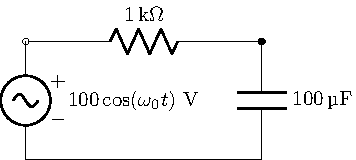
\includegraphics[width = 0.5\columnwidth]{2023/BM/16/figs/c_fig1.pdf}
    \caption{circuit }
    \centering
    \label{fig: bm_16_fig_1}
\end{figure}
\begin{enumerate}
    \item[(A)] 1000
    \item[(B)] 100
    \item[(C)] 1
    \item[(D)] 0   
\end{enumerate}
\hfill(GATE BM 2023 Question 16)\\

\solution
\iffalse
\let\negmedspace\undefined
\let\negthickspace\undefined
\documentclass[journal,12pt,twocolumn]{IEEEtran}
\usepackage{cite}
\usepackage{amsmath,amssymb,amsfonts,amsthm}
\usepackage{algorithmic}
\usepackage{graphicx}
\usepackage{textcomp}
\usepackage{xcolor}
\usepackage{txfonts}
\usepackage{listings}
\usepackage{enumitem}
\usepackage{mathtools}
\usepackage{gensymb}
\usepackage{comment}
\usepackage[breaklinks=true]{hyperref}
\usepackage{tkz-euclide}
\usepackage{listings}
\usepackage{gvv}
\def\inputGnumericTable{}
\usepackage[latin1]{inputenc}
\usepackage{color}
\usepackage{array}
\usepackage{longtable}
\usepackage{calc}
\usepackage{multirow}
\usepackage{hhline}
\usepackage{ifthen}
\usepackage{lscape}

\newtheorem{theorem}{Theorem}[section]
\newtheorem{problem}{Problem}
\newtheorem{proposition}{Proposition}[section]
\newtheorem{lemma}{Lemma}[section]
\newtheorem{corollary}[theorem]{Corollary}
\newtheorem{example}{Example}[section]
\newtheorem{definition}[problem]{Definition}
\newcommand{\BEQA}{\begin{eqnarray}}
\newcommand{\EEQA}{\end{eqnarray}}
\newcommand{\define}{\stackrel{\triangle}{=}}
\theoremstyle{remark}
\newtheorem{rem}{Remark}
\begin{document}

\bibliographystyle{IEEEtran}
\vspace{3cm}

\title{GATE -BM 16}
\author{EE23BTECH11057 - Shakunaveti Sai Sri Ram Varun$^{}$% &lt;-this % stops a space
}
\maketitle
\newpage
\bigskip
\vspace{2cm}
\textbf{Question: }
For the circuit given below, choose the angular frequency $ \omega_0$ at which voltage across capacitor has maximum amplitude?
\begin{figure}[h!]
    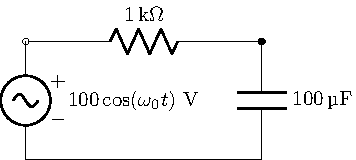
\includegraphics[width = \columnwidth]{2023/BM/16/figs/c_fig1.pdf}
    \caption{circuit }
    \centering
    \label{fig: bm_16_fig_1}
\end{figure}\\
\begin{enumerate}
    \item[(A)] 1000\\
    \item[(B)] 100\\
    \item[(C)] 1\\
    \item[(D)] 0   
\end{enumerate}
\hfill(GATE BM 2023 question 16)\\
\textbf{Solution}:\\
\fi
\begin{table}[h!] 
\centering
\begin{tabular}{|c|c|c|}
    \hline
    \textbf{Parameter} & \textbf{Description} & \textbf{Value} \\
    \hline
    $V_i(j\omega)$ & Input voltage & $100$ \\
    \hline
    $v_c(t)$ & Potential difference across Capacitor & ? \\
    \hline
    $V_c(s)$ & Potential difference across Capacitor & $V_c(s)$ \\
    \hline
    $H(s)$ & Transfer function & $\frac{V_c(s)}{V_i(s)}$ \\
    \hline
    $V_o$ & Amplitude of input voltage & $100 \, \text{V}$ \\
    \hline
    $R$ & Resistance in circuit & $1 \, \text{k}\Omega$ \\
    \hline
    $C$ & Capacitance in circuit & $100 \, \mu\text{F}$ \\
    \hline
    $\omega_o$ & Angular frequency of input voltage & $\omega_o$ \\
    \hline
\end{tabular}


\caption{input values}
\label{tab: table-bm16}
\end{table}

\begin{align}
V_c\brak{s}&= \frac{V_1\brak{s}\frac{1}{sC}}{R+\frac{1}{sC}}\\
\implies H\brak{s} &= \frac{1}{1+ sRC}\\
\implies H\brak{j\omega} &= \frac{1}{1+j\omega RC}\\
|H\brak{j\omega}| &= \frac{1}{\sqrt{1+\brak{\omega RC}^2}}
\end{align}
\begin{figure}[h!]
    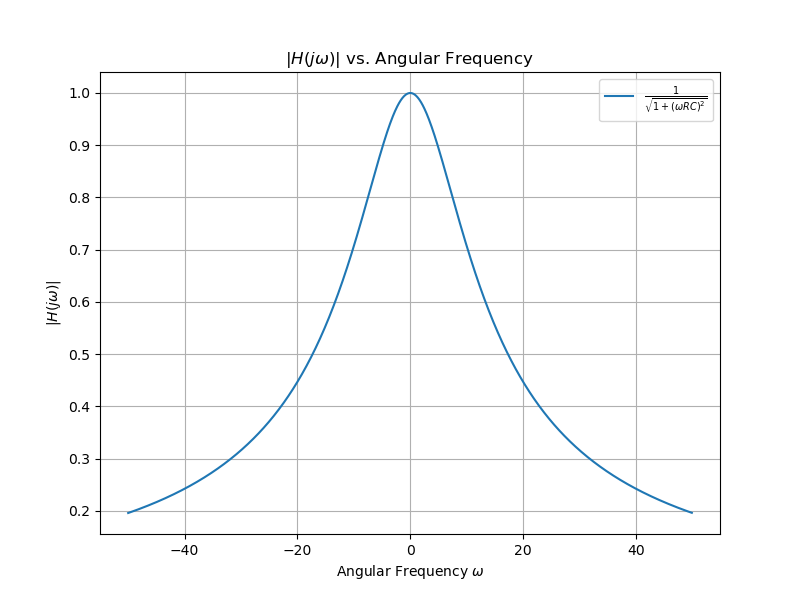
\includegraphics[width = \columnwidth]{2023/BM/16/figs/Figure_1.png}
    \caption{$ |H\brak{j\omega}|$ }
    \centering
    \label{fig: bm_16_fig_2}
\end{figure}


\begin{figure}[h!]
    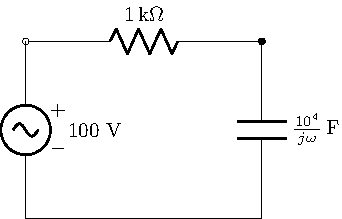
\includegraphics[width = \columnwidth]{2023/BM/16/figs/c_fig2.pdf}
    \caption{circuit in $ \omega$-domain }
    \centering
    \label{fig: bm_16_fig_3}
\end{figure}

\begin{align}
v_c\brak{t}&= \frac{100}{\sqrt{1+\brak{\omega_o RC}^2}}\brak{\cos{\omega_o t + \arctan\brak{\frac{1}{\omega_o RC}}}}
\end{align}
Maximum amplitude of $ v_c\brak{t}$ occurs at $ \omega_o=0$
\begin{align}
\therefore \omega_o =0
\end{align}
$ \therefore$ maximum value of $ v_c\brak{t}$ at steady state is $ 100$ Volts.

\newpage
\item
In the following circuit, the switch S is open for $t < 0$ and closed for $t \ge 0$.
What is the steady state voltage (in Volts) across the capacitor when the switch is closed?
\begin{figure}[h!]
    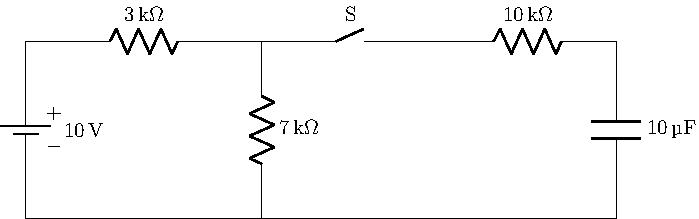
\includegraphics[width = 0.7\columnwidth]{2023/BM/30/figs/c_fig1.pdf}
    \caption{circuit }
    \centering
    \label{fig:bm_30_fig_1}
\end{figure}
\hfill(GATE BM 2023 Question 30)\\
\item 
A finite impulse response (FIR) filter has only two non-zero samples in its impulse response $h[n]$, namely $h[0] = h[1] = 1$. The Discrete Time Fourier Transform (DTFT) of $h[n]$ equals $H(e^{j\omega})$, as a function of the normalized angular frequency $\omega$. For the range $\abs{\omega} \leq \pi$, $\abs{H(e^{j\omega})}$ is equal to
\begin{enumerate}
	\item[(A)] $2\abs{\cos(\omega)}$
	\item[(B)] $2\abs{\sin(\omega)}$
	\item[(C)] $2\abs{\cos(\frac{\omega}{2})}$
	\item[(D)] $2\abs{\sin(\frac{\omega}{2})}$
\end{enumerate}
\hfill(GATE BM 2023 Question 17) \\
\solution
\let\negmedspace\undefined
\let\negthickspace\undefined
\documentclass[journal,12pt,onecolumn]{IEEEtran}
\usepackage{cite}
\usepackage{amsmath,amssymb,amsfonts,amsthm}
%\usepackage{algorithmic}
\usepackage{graphicx}
\usepackage{textcomp}
\usepackage{xcolor}
\usepackage{txfonts}
\usepackage{listings}
\usepackage{enumitem}
\usepackage{mathtools}
\usepackage{gensymb}
\usepackage[breaklinks=true]{hyperref}
\usepackage{tkz-euclide} % loads  TikZ and tkz-base
\usepackage{listings}
\usepackage{float}



\newtheorem{theorem}{Theorem}[section]
\newtheorem{problem}{Problem}
\newtheorem{proposition}{Proposition}[section]
\newtheorem{lemma}{Lemma}[section]
\newtheorem{corollary}[theorem]{Corollary}
\newtheorem{example}{Example}[section]
\newtheorem{definition}[problem]{Definition}
%\newtheorem{thm}{Theorem}[section] 
%\newtheorem{defn}[thm]{Definition}
%\newtheorem{algorithm}{Algorithm}[section]
%\newtheorem{cor}{Corollary}
\newcommand{\BEQA}{\begin{eqnarray}}
\newcommand{\EEQA}{\end{eqnarray}}
\newcommand{\define}{\stackrel{\triangle}{=}}
\theoremstyle{remark}
\newtheorem{rem}{Remark}
%\bibliographystyle{ieeetr}
\begin{document}
%
\providecommand{\pr}[1]{\ensuremath{\Pr\left(#1\right)}}
\providecommand{\prt}[2]{\ensuremath{p_{#1}^{\left(#2\right)} }}        % own macro for this question
\providecommand{\qfunc}[1]{\ensuremath{Q\left(#1\right)}}
\providecommand{\sbrak}[1]{\ensuremath{{}\left[#1\right]}}
\providecommand{\lsbrak}[1]{\ensuremath{{}\left[#1\right.}}
\providecommand{\rsbrak}[1]{\ensuremath{{}\left.#1\right]}}
\providecommand{\brak}[1]{\ensuremath{\left(#1\right)}}
\providecommand{\lbrak}[1]{\ensuremath{\left(#1\right.}}
\providecommand{\rbrak}[1]{\ensuremath{\left.#1\right)}}
\providecommand{\cbrak}[1]{\ensuremath{\left\{#1\right\}}}
\providecommand{\lcbrak}[1]{\ensuremath{\left\{#1\right.}}
\providecommand{\rcbrak}[1]{\ensuremath{\left.#1\right\}}}
\newcommand{\sgn}{\mathop{\mathrm{sgn}}}
\providecommand{\abs}[1]{\left\vert#1\right\vert}
\providecommand{\res}[1]{\Res\displaylimits_{#1}} 
\providecommand{\norm}[1]{\left\lVert#1\right\rVert}
%\providecommand{\norm}[1]{\lVert#1\rVert}
\providecommand{\mtx}[1]{\mathbf{#1}}
\providecommand{\mean}[1]{E\left[ #1 \right]}
\providecommand{\cond}[2]{#1\middle|#2}
\providecommand{\fourier}{\overset{\mathcal{F}}{ \rightleftharpoons}}
\newenvironment{amatrix}[1]{%
  \left(\begin{array}{@{}*{#1}{c}|c@{}}
}{%
  \end{array}\right)
}
%\providecommand{\hilbert}{\overset{\mathcal{H}}{ \rightleftharpoons}}
%\providecommand{\system}{\overset{\mathcal{H}}{ \longleftrightarrow}}
	%\newcommand{\solution}[2]{\textbf{Solution:}{#1}}
\newcommand{\solution}{\noindent \textbf{Solution: }}
\newcommand{\cosec}{\,\text{cosec}\,}
\providecommand{\dec}[2]{\ensuremath{\overset{#1}{\underset{#2}{\gtrless}}}}
\newcommand{\myvec}[1]{\ensuremath{\begin{pmatrix}#1\end{pmatrix}}}
\newcommand{\mydet}[1]{\ensuremath{\begin{vmatrix}#1\end{vmatrix}}}
\newcommand{\myaugvec}[2]{\ensuremath{\begin{amatrix}{#1}#2\end{amatrix}}}
\providecommand{\rank}{\text{rank}}
\providecommand{\pr}[1]{\ensuremath{\Pr\left(#1\right)}}
\providecommand{\qfunc}[1]{\ensuremath{Q\left(#1\right)}}
	\newcommand*{\permcomb}[4][0mu]{{{}^{#3}\mkern#1#2_{#4}}}
\newcommand*{\perm}[1][-3mu]{\permcomb[#1]{P}}
\newcommand*{\comb}[1][-1mu]{\permcomb[#1]{C}}
\providecommand{\qfunc}[1]{\ensuremath{Q\left(#1\right)}}
\providecommand{\gauss}[2]{\mathcal{N}\ensuremath{\left(#1,#2\right)}}
\providecommand{\diff}[2]{\ensuremath{\frac{d{#1}}{d{#2}}}}
\providecommand{\myceil}[1]{\left \lceil #1 \right \rceil }
\newcommand\figref{Fig.~\ref}
\newcommand\tabref{Table~\ref}
\newcommand{\sinc}{\,\text{sinc}\,}
\newcommand{\rect}{\,\text{rect}\,}
%%
%	%\newcommand{\solution}[2]{\textbf{Solution:}{#1}}
%\newcommand{\solution}{\noindent \textbf{Solution: }}
%\newcommand{\cosec}{\,\text{cosec}\,}
%\numberwithin{equation}{section}
%\numberwithin{equation}{subsection}
%\numberwithin{problem}{section}
%\numberwithin{definition}{section}
%\makeatletter
%\@addtoreset{figure}{problem}
%\makeatother

%\let\StandardTheFigure\thefigure
\let\vec\mathbf

\bibliographystyle{IEEEtran}





\bigskip

%\renewcommand{\thefigure}{\theenumi}
%\renewcommand{\thetable}{\theenumi}
%\renewcommand{\theequation}{\theenumi}

A finite impulse response (FIR) filter has only two non-zero samples in its impulse response $h[n]$, namely $h[0] = h[1] = 1$. The Discrete Time Fourier Transform (DTFT) of $h[n]$ equals $H(e^{j\omega})$, as a function of the normalized angular frequency $\omega$. For the range $\abs{\omega} \leq \pi$, $\abs{H(e^{j\omega})}$ is equal to
\begin{enumerate}
	\item[(A)] $2\abs{\cos(\omega)}$
	\item[(B)] $2\abs{\sin(\omega)}$
	\item[(C)] $2\abs{\cos(\frac{\omega}{2})}$
	\item[(D)] $2\abs{\sin(\frac{\omega}{2})}$
\end{enumerate}
\hfill(GATE BM 2023)

\solution
\begin{table}[H]
	\centering
\begin{tabular}{|c|c|c|}
	\hline
	\textbf{Parameter} & \textbf{Value} & \textbf{Description} \\
	\hline
	$h[n]$ & - & impulse response \\
	\hline
	$h[0]$ & 1 & impulse response at $n=0$ \\
	\hline
	$h[1]$ & 1 & impulse response at $n=1$ \\
	\hline
	$\omega$ & $-\pi\leq\omega\leq\pi$ & normalized frequency \\
	\hline
	$H(e^{j\omega})$ & $\sum_{n=0}^{M} h[n]e^{-jn\omega}$ & frequency response \\
    	\hline
\end{tabular}
\caption{Input Parameters Table}
\label{tab:gate23bm17.1}

\end{table}
From \tabref{tab:gate23bm17.1},
\begin{align}
	H(e^{j\omega}) &= 1 + e^{-j\omega} \\
	&= e^{\frac{-j\omega}{2}}(e^{\frac{j\omega}{2}} + e^{\frac{-j\omega}{2}}) \\
	&= e^{\frac{-j\omega}{2}}(2\cos{\brak{\frac{\omega}{2}}}) \\
	\abs{H(e^{j\omega})} &= 2\abs{\cos{\brak{\frac{\omega}{2}}}}
\end{align}

\begin{figure}[ht]
	\centering
	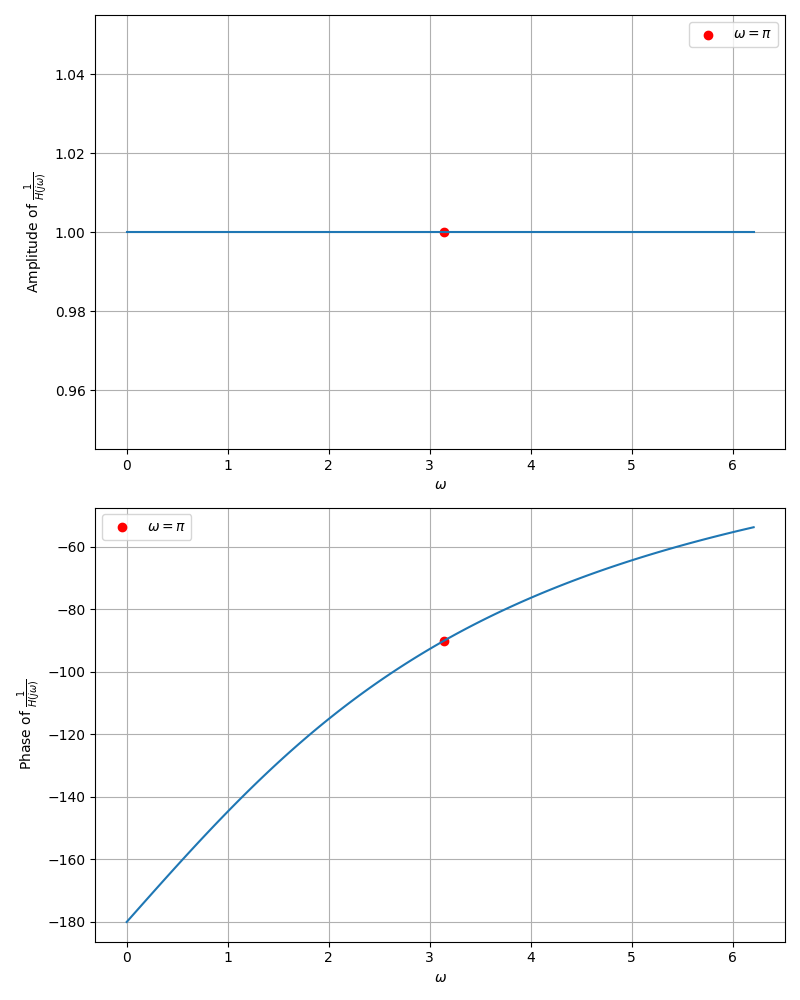
\includegraphics[width=0.8\textwidth]{./figs/fig1.png}
\end{figure}
\end{document}

\pagebreak
\item
For the circuit shown,if $i=\sin 1000t$, the instantaneous value of the Thevenin's voltage(in volts) across the terminals a anb b at time t=5ms is\\[2pt]

\begin{circuitikz}[american voltages,american currents]
    % Draw the circuit components
    \draw (0,0) -- (2,0);
    \draw (2,2) to [resistor,l=$10\Omega$] (2,4);
    \draw (2,4) -- (0,4);
    \draw (2,0) to [capacitor,l=$-j10\Omega$,-,i_=$i_x$] (2,2);
    \draw (2,0) -- (5,0);
    \draw (5,0) to[inductor,l=$j10\Omega$] (5,2);
    \draw (5,2) to [resistor,l=$10\Omega$] (5,4);
  \draw (5,4) to [cV,l^=$4i_x$,invert] (2,4);
  \draw (5,4) -- (6,4);
  \draw (6,4) to[I,l=$\sin 1000t$,invert] (6,0);
  \draw (6,0) -- (5,0);
   \node[circle,fill=black,inner sep=1.5pt,label=above:a] at (0,0) {};
    \node[circle,fill=black,inner sep=1.5pt,label=above:b] at (0,4) {};
    \end{circuitikz}
    \hfill(GATE EE 2023 Question 51) \\
    \pagebreak

    \item In the circuit shown ,$\omega=100\pi\text{rads/s}$, R1=R2=$2.2\Omega$ and L=$7\text{mH}$. the capacitance $\text{C}$ for which $Y_{in}$ is purely real is  $\text{mF}$ \\
	\begin{center}
	\begin{circuitikz} \centering \draw 
		(0,4) to[sinusoidal voltage source, l=$V_{0}$cos($\omega$t)] (0,0)
		(0,4) to[short] (4,4)
		(4,4) to[resistor, l=$R_1$ ] (4,2)
		(4,2) to[inductor, l= $\text{L} $] (4,0) to[short ] (0,0)
		(8,4)  to[short] (4,4)
		(8,4) to[resistor, l= $R_2$] (8,2) to[capacitor,l=$\text{C}$] (8,0) to (4,0);
	\end{circuitikz}
	\end{center}
\hfill(GATE IN 2023 Q46)\\
\solution
\iffalse
\let\negmedspace\undefined
\let\negthickspace\undefined
\documentclass[a4,12pt,onecolumn]{IEEEtran}
\usepackage{amsmath,amssymb,amsfonts,amsthm}
\usepackage{algorithmic}
\usepackage{graphicx}
\usepackage{textcomp}
\usepackage{xcolor}
\usepackage{txfonts}
\usepackage{listings}
\usepackage{enumitem}
\usepackage{mathtools}
\usepackage{gensymb}
\usepackage[breaklinks=true]{hyperref}
\usepackage{tkz-euclide}
\usepackage{listings}
\usepackage{circuitikz}
\usepackage{gvv}
\begin{document}
\title{
\Huge\textbf{ GATE 2023 Assignment}\\
\Huge\textbf{EE1205} Signals and Systems\\
}
\large\author{Kurre Vinay\\EE23BTECH11036}
\maketitle
\textbf{Question:}
In the circuit shown ,$\omega=100\pi\text{rads/s}$, $R_1$=$R_2$=$2.2\Omega$ and $L$=$7\text{mH}$. the capacitance $\text{C}$ for which $Y_{in}$ is purely real is \underline{\hspace{1cm}}  $\text{mF}$ \\
	\begin{center}
	\begin{circuitikz} \centering \draw 
		(0,4) to[sinusoidal voltage source, l=$V_{0}$cos($\omega$t)] (0,0)
		(0,4) to[short] (4,4)
		(4,4) to[resistor, l=$R_1$ ] (4,2)
		(4,2) to[inductor, l= $\text{L} $] (4,0) to[short ] (0,0)
		(8,4)  to[short] (4,4)
		(8,4) to[resistor, l= $R_2$] (8,2) to[capacitor,l=$\text{C}$] (8,0) to (4,0);
	\end{circuitikz}
	\end{center}
\hfill(GATE IN 2023 )\\
\solution\\
\fi
\begin{table}[ht!]
\begin{center}

\begin{tabular}{|c|c|c|c|}
   \hline
   variable&value&description&formulae \\
   \hline
   $Y_{in}$ & -& Admittance of circuit&$\frac{R_1-Ls}{R_1^2-\brak{Ls}^2} + \frac{R_2-\frac{1}{ \text{sC}}}{R_2^2-\brak{\frac{1}{ \text{sC}}}^2}$\\
   \hline
   $X_{L}$ & $7s\Omega$ & Inductive reactance&$\text{sL}$ \\
   \hline
   $X_{C}$ &$\frac{1}{s\text{C}}\Omega $ & Capacitive reactance& $\frac{1}{s\text{C}}$\\
   \hline
    $\text{s}$& $100\pi\text{j}$&Laplace complex frequency&$j\omega$\\
   \hline
   $\omega$ &$100\pi$rads/s& Angular frequency&-\\
   \hline
   $\text{V}$&$V_{0}$cos($\omega$t)&voltage of source&-\\
   \hline
   $R_1 , R_2$& $2.2\Omega$ &resistance of resistors&-\\
   \hline
 
\end{tabular}
\caption{Table: Input Parameters}
\label{tab:1.46Q}
\end{center}
\end{table}
\\From $\tabref{tab:1.46Q}$
\begin{align} 
Y_{in}&=\frac{R_1-Ls}{R_1^2-\brak{Ls}^2} + \frac{R_2-\frac{1}{ \text{sC}}}{R_2^2-\brak{\frac{1}{ \text{sC}}}^2}\\
Im\brak{Y_{in}}&=\frac{-Ls}{R_1^2-\brak{Ls}^2} + \frac{-\frac{1}{ \text{sC}}}{R_2^2-\brak{\frac{1}{ \text{sC}}}^2}
\end{align}
According to the question given, $Y_{in}$ is purely real , so imaginary part should be equal to zero\\
Take the values from $\tabref{tab:1.46Q}$\\
\begin{align}
 \frac{-1}{4.4}+\frac{\frac{1}{ (100\pi) \text{C}}}{(2.2)^2+\brak{\frac{1}{ (100\pi) \text{C}}}^2}&=0\\ 
 \frac{\frac{1}{ (100\pi) \text{C}}}{(2.2)^2+\brak{\frac{1}{ (100\pi) \text{C}}}^2}&=\frac{1}{4.4}\\
  (2.2)^2-\frac{4.4}{ (100\pi) \text{C}}+\brak{\frac{1}{ (100\pi) \text{C}}}^2&=0\\
 \brak{2.2-\frac{1}{ (100\pi) \text{C}}}^2&=0\\
 \frac{1}{ (100\pi) \text{C}}&=2.2\\
 \text{C}&=\frac{700}{484}\text{mF}\\
 \text{C}&=1.446281\text{mF}
\end{align}
The capacitance of capacitor $\text{C}$ is 1.45$\text{mF}$
\begin{figure}[ht!]
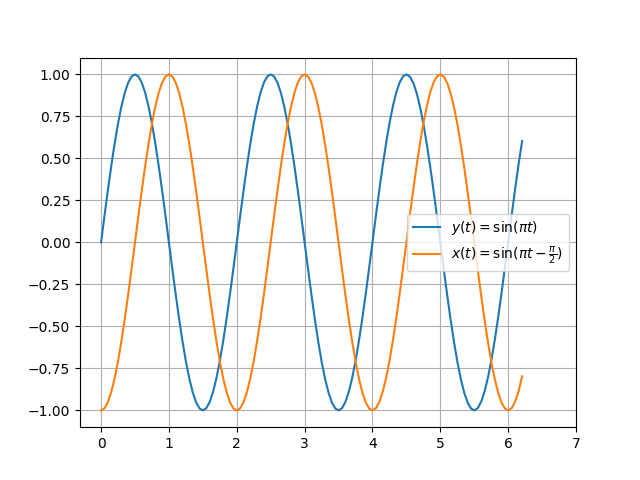
\includegraphics[width=\columnwidth]{figs/fig2.png}
\caption{\large{the plot of capacitance vs magnitude of $Y_{in}$}}
\end{figure}

\end{document}


\pagebreak
\item An input voltage in the form of a square wave of frequency $1\, kHz$ is given to a circuit, which results in the output shown schematically below. Which one of the following options is the CORRECT representation of the circuit? \hfill(GATE PH 2023 Q37)
\begin{figure}[!h]
    \centering
    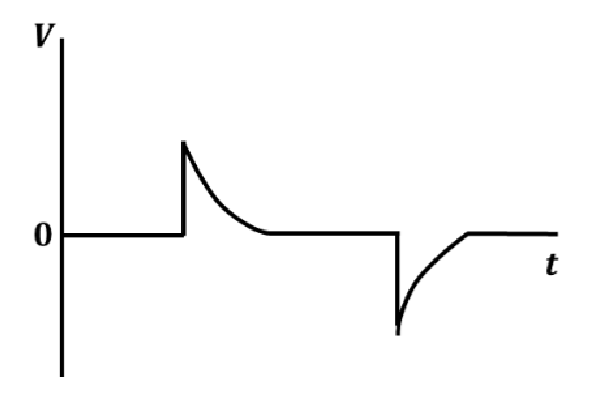
\includegraphics[width = 0.6\columnwidth]{2023/PH/37/figs/question.png}
	\caption{}\
	\label{fig:ques_gate.ph.23.37}
\end{figure}

\begin{enumerate}[label = (\alph*)]
    \item 
    \begin{figure}[!h]
        \centering
	    \resizebox{0.2\textwidth}{!}{\begin{circuitikz}
    \draw(0, 0) to[short,*-*] ++ (4,0);
\draw (0,2) to[C,l=$0.1\mu F$, *-*] ++ (3,0) coordinate(a);
\draw (a) to[short,-*] ++ (1,0);
\draw (a) to[R, l_=$0.5k\Omega$,*-] ++(0,-2);

% Voltage labels
\draw (0,2) to[open,l_=V$_{in}$] ++(0,-2);
\draw (4,2) to[open,l=V$_{out}$] ++(0,-2);
\end{circuitikz}

}
	\label{optA_gate.ph.23.37}
    \end{figure}

    \item 
    \begin{figure}[!h]
        \centering
        \resizebox{0.2\textwidth}{!}{\begin{circuitikz}
    \draw(0, 0) to[short,*-*] ++ (4,0);
\draw (0,2) to[C,l=$1\mu F$, *-*] ++ (3,0) coordinate(a);
\draw (a) to[short,-*] ++ (1,0);
\draw (a) to[R, l_=$5k\Omega$,*-] ++(0,-2);

% Voltage labels
\draw (0,2) to[open,l_=V$_{in}$] ++(0,-2);
\draw (4,2) to[open,l=V$_{out}$] ++(0,-2);
\end{circuitikz}

}
        \label{optB_gate.ph.23.37}
    \end{figure}

    \item 
    \begin{figure}[!h]
        \centering
        \resizebox{0.2\textwidth}{!}{\begin{circuitikz}
    \draw(0, 0) to[short,*-*] ++ (4,0);
\draw (0,2) to[R, l = $0.5k\Omega$, *-] ++ (3,0) coordinate(a);
\draw (a) to[short,-*] ++ (1,0);
\draw (a) to[C,l_=$0.1\mu F$,*-*] ++(0,-2);

% Voltage labels
\draw (0,2) to[open,l_=V$_{in}$] ++(0,-2);
\draw (4,2) to[open,l=V$_{out}$] ++(0,-2);
\end{circuitikz}

}
        \label{optC_gate.ph.23.37}
    \end{figure}

    \item 
    \begin{figure}[!h]
        \centering
        \resizebox{0.2\textwidth}{!}{\begin{circuitikz}
    \draw(0, 0) to[short,*-*] ++ (4,0);
\draw (0,2) to[R, l = $5k\Omega$, *-] ++ (3,0) coordinate(a);
\draw (a) to[short,-*] ++ (1,0);
\draw (a) to[C,l_=$1\mu F$,*-*] ++(0,-2);

% Voltage labels
\draw (0,2) to[open,l_=V$_{in}$] ++(0,-2);
\draw (4,2) to[open,l=V$_{out}$] ++(0,-2);
\end{circuitikz}

}
        \label{optD_gate.ph.23.37}
    \end{figure}
\end{enumerate} \hfill(GATE 2023 PH 37)\\
\solution
\iffalse
\let\negmedspace\undefined
\let\negthickspace\undefined
\documentclass[journal,12pt,twocolumn]{IEEEtran}
\usepackage{cite}
\usepackage{amsmath,amssymb,amsfonts,amsthm}
\usepackage{algorithmic}
\usepackage{graphicx}
\usepackage{textcomp}
\usepackage{xcolor}
\usepackage{txfonts}
\usepackage{listings}
\usepackage{enumitem}
\usepackage{mathtools}
\usepackage{gensymb}
\usepackage{comment}
\usepackage[breaklinks=true]{hyperref}
\usepackage{tkz-euclide} 
\usepackage{listings}
\usepackage{gvv}                            \usepackage{tikz}
\usepackage{circuitikz}
\def\inputGnumericTable{}                                
\usepackage[latin1]{inputenc}                            
\usepackage{color}                                       
\usepackage{array}                                       
\usepackage{longtable}                                   
\usepackage{calc}                              
\usepackage{tikz}
\usepackage{multirow}                                    
\usepackage{hhline}                                      
\usepackage{ifthen}                            
\usepackage{caption}
\usepackage{lscape}
\usepackage{amsmath}
\newtheorem{theorem}{Theorem}[section]
\newtheorem{problem}{Problem}
\newtheorem{proposition}{Proposition}[section]
\newtheorem{lemma}{Lemma}[section]
\newtheorem{corollary}[theorem]{Corollary}
\newtheorem{example}{Example}[section]
\newtheorem{definition}[problem]{Definition}
\newcommand{\BEQA}{\begin{eqnarray}}
\newcommand{\EEQA}{\end{eqnarray}}
\newcommand{\define}{\stackrel{\triangle}{=}}
\theoremstyle{remark}
\newtheorem{rem}{Remark}

\begin{document}

\bibliographystyle{IEEEtran}
\vspace{3cm}

\title{GATE 2023 PH Q37}
\author{EE23BTECH11009 - AROSHISH PRADHAN$^{*}$% <-this % stops a space
}
\maketitle
\newpage
\bigskip
\textbf{Question:} An input voltage in the form of a square wave of frequency $1\, kHz$ is given to a circuit, which results in the output shown schematically below. Which one of the following options is the CORRECT representation of the circuit?

\begin{figure}[!h]
    \centering
    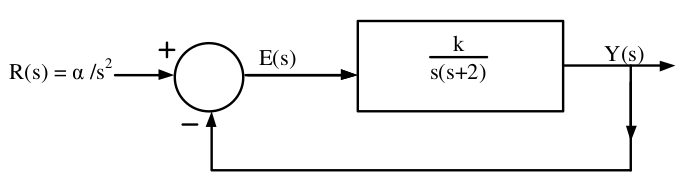
\includegraphics[width = \columnwidth]{figs/question.png}
    \caption{}
    \label{fig:ques_gate.ph.23.37}
\end{figure}

\begin{enumerate}[label = (\alph*)]
    \item
    \begin{minipage}[t]{\columnwidth}
        \begin{circuitikz}
    \draw(0, 0) to[short,*-*] ++ (4,0);
\draw (0,2) to[C,l=$0.1\mu F$, *-*] ++ (3,0) coordinate(a);
\draw (a) to[short,-*] ++ (1,0);
\draw (a) to[R, l_=$0.5k\Omega$,*-] ++(0,-2);

% Voltage labels
\draw (0,2) to[open,l_=V$_{in}$] ++(0,-2);
\draw (4,2) to[open,l=V$_{out}$] ++(0,-2);
\end{circuitikz}


    \end{minipage}
    \item
    \begin{minipage}[t]{\columnwidth}
        \begin{circuitikz}
    \draw(0, 0) to[short,*-*] ++ (4,0);
\draw (0,2) to[C,l=$1\mu F$, *-*] ++ (3,0) coordinate(a);
\draw (a) to[short,-*] ++ (1,0);
\draw (a) to[R, l_=$5k\Omega$,*-] ++(0,-2);

% Voltage labels
\draw (0,2) to[open,l_=V$_{in}$] ++(0,-2);
\draw (4,2) to[open,l=V$_{out}$] ++(0,-2);
\end{circuitikz}


    \end{minipage}
    \item
    \begin{minipage}[t]{\columnwidth}
        \begin{circuitikz}
    \draw(0, 0) to[short,*-*] ++ (4,0);
\draw (0,2) to[R, l = $0.5k\Omega$, *-] ++ (3,0) coordinate(a);
\draw (a) to[short,-*] ++ (1,0);
\draw (a) to[C,l_=$0.1\mu F$,*-*] ++(0,-2);

% Voltage labels
\draw (0,2) to[open,l_=V$_{in}$] ++(0,-2);
\draw (4,2) to[open,l=V$_{out}$] ++(0,-2);
\end{circuitikz}


    \end{minipage}
    \item
    \begin{minipage}[t]{\columnwidth}
        \begin{circuitikz}
    \draw(0, 0) to[short,*-*] ++ (4,0);
\draw (0,2) to[R, l = $5k\Omega$, *-] ++ (3,0) coordinate(a);
\draw (a) to[short,-*] ++ (1,0);
\draw (a) to[C,l_=$1\mu F$,*-*] ++(0,-2);

% Voltage labels
\draw (0,2) to[open,l_=V$_{in}$] ++(0,-2);
\draw (4,2) to[open,l=V$_{out}$] ++(0,-2);
\end{circuitikz}


    \end{minipage}
\end{enumerate}

\solution
\fi
\begin{table}[!h]
    \centering
    \begin{tabular}{|c|c|c|}
    \hline
       \textbf{Symbol}  & \textbf{Value} &  \textbf{Description}\\
    \hline
       $V_{in}(t)$  &  &  Input Voltage\\
    \hline
        $\mathcal{V}_{in}(f)$ & & Fourier Transform of $V_{in}(t)$\\
    \hline
        $V_{out}(t)$ & & Output Voltage\\
    \hline
        $\mathcal{V}_{out}(f)$ & & Fourier Transform of $V_{out}(t)$\\
    \hline
        $f$ & $1000Hz$ & Input Wave Frequency\\
    \hline
        $T$ & $\dfrac{1}{f} = 10^{-3} s$ & Input Wave Time Period\\
    \hline
        \multirow{2}{*}{$R$} & (a) $0.5k\Omega$ & \multirow{2}{*}{Resistance}\\
        \cline{2-2}
        & (b) $5k\Omega$ &\\
        \cline{2-2}
    \hline
        \multirow{2}{*}{$C$} & (a) $0.1\mu F$ & \multirow{2}{*}{Capacitance}\\
        \cline{2-2}
        & (b) $1\mu F$ &\\
        \cline{2-2}
    \hline
        $\tau$ & $RC$ & Time Constant\\
    \hline
        $Z$ & $R + \frac{1}{sC}$ & Impedance\\
    \hline
        $H(f)$ & $\frac{V_{out}}{V_{in}}$ & General Transfer Function\\
    \hline
        $H_{R}(f)$ & $\frac{V_{R, out}}{V_{in}}$ & Transfer Function for Resistor\\
    \hline
        $H_{C}(f)$ & $\frac{V_{C, out}}{V_{in}}$ & Transfer Function for Capacitor\\
    \hline
    \end{tabular}
    \caption{Given Parameters}
    \label{tab:1_gate.23.ph.37}
\end{table}


Input waveform is a square wave (\figref{fig:square_gate.ph.23.37}), so we take its Fourier Transform 
\begin{align}
    V_{in}(t) &= 2\brak{2\sbrak{\frac{\brak{t-\frac{T}{4}}}{T}} - \sbrak{\frac{2\brak{t - \frac{T}{4}}}{T}}} + 1
\end{align}
Fourier Series Coefficient:
\begin{align}
    c_k = \frac{1}{T} \int_{T} V_{in}(t)e^{-jk\omega t}dt
\end{align}
As square wave is even, $\sin(k\omega t)$ terms become zero. Cosine coefficients are:
\begin{align}
    a_n &= \frac{2}{T} \int_{T} V_{in}(t) \cos\brak{\frac{2\pi nt}{T}}\\
    &= \frac{4}{n\pi}\sin{\brak{\frac{n\pi}{2}}}\cos\brak{{n\pi}}
\end{align}

Fourier Series of $V_{in}(t)$:
\begin{align}
    V_{in}(t) = \sum_{n = 1}^{\infty}a_n \cos\brak{\frac{2\pi nt}{T}}\label{eq:5_gate.23.ph.37}
\end{align}

\begin{figure}[!h]
    \centering
    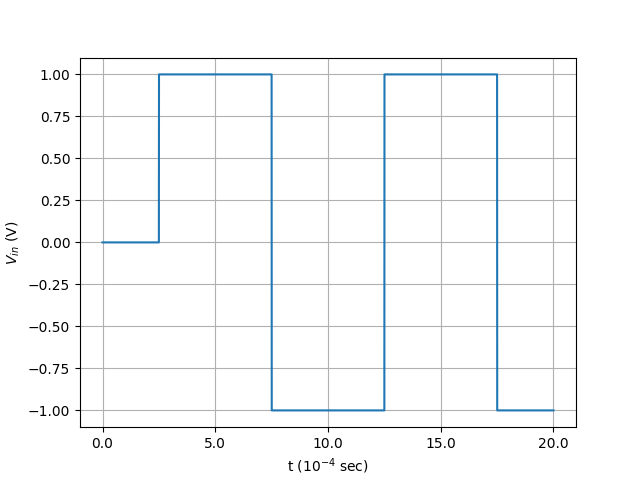
\includegraphics[width = \columnwidth]{2023/PH/37/figs/square.png}
    \caption{Input Square Waveform ($V_{in}(t)$)}
    \label{fig:square_gate.ph.23.37}
\end{figure}

Taking Fourier Transform of $V_{in}(t)$:
\begin{align}
    V_{in}(t) &\system{F} \mathcal{V}_{in}(j\omega)
\end{align}

\begin{figure}[!h]
    \centering
    \begin{circuitikz}
    \draw(0, 0) to[short,*-] ++ (3,0);
    \draw (0,2) to[C,l=$\frac{1}{sC}$, *-] ++ (3,0) coordinate(a);
    %\draw (a) to[short,-*] ++ (1,0);
    \draw (a) to[R, l_=$R$,*-] ++(0,-2);
    
    % Voltage labels
    \draw (0,2) to[open,l_=V$_{in}$] ++(0,-2);
    \end{circuitikz}
    \caption{Series RC Circuit in s-domain}
    \label{fig:s-domain_gate.ph.23.37}
\end{figure}

\begin{align}
    s &= j\omega\\
    \implies Z &= R + \frac{1}{sC}\\
    &= R + \frac{1}{j\omega C}
\end{align}

$\mathcal{V}_{in}(j\omega)$ was input into all four circuits and $V_{out}(t)$ was calculated using the Transfer Functions of the $RC$ Filters.

Transfer Function:
\begin{align}
    H(j\omega) &= \frac{V_{out}}{V_{in}}
\end{align}
\begin{enumerate}
    \item Option A
    \begin{align}
        H_R(j\omega) &=  \frac{R}{R + \frac{1}{j\omega C}}\\
        &= \frac{j\omega RC}{1+j\omega RC}\\
        &= \brak{\frac{\omega R C}{\sqrt{1 + (\omega R C)^2}}}e^{j\tan^{-1}\brak{\frac{1}{\omega RC}}}\label{eq:13_gate.23.ph.37}
    \end{align}
    \begin{figure}[!h]
        \centering
        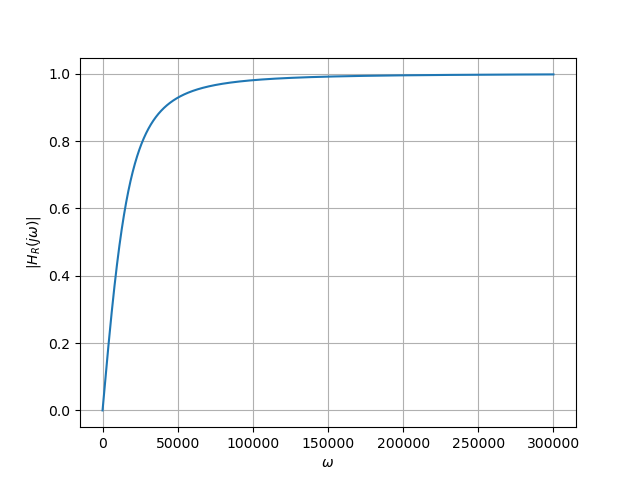
\includegraphics[width=\columnwidth]{2023/PH/37/figs/opt_a_hf.png}
        \caption{$\abs{H_R(j\omega)}$ vs $\omega$ for $R=0.5k\Omega$, $C=0.1\mu F$}
        \label{fig:opt_a_hf_gate.ph.23.37}
    \end{figure}
    \begin{align}
        \implies \mathcal{V}_{out}(j\omega) &= H_R(j\omega)\mathcal{V}_{in}(j\omega)\\
    \end{align}
    Using \eqref{eq:5_gate.23.ph.37} and  \eqref{eq:13_gate.23.ph.37},
    {\small
    \begin{align}
        V_{out}(t) &= \sum_{n=1}^{\infty}\brak{\frac{n\omega R C}{\sqrt{1 + (n\omega R C)^2}}}a_n\cos\brak{n\omega t+\tan^{-1}\brak{\frac{1}{n\omega RC}}}
    \end{align}
    }
    \begin{figure}[!h]
        \centering
        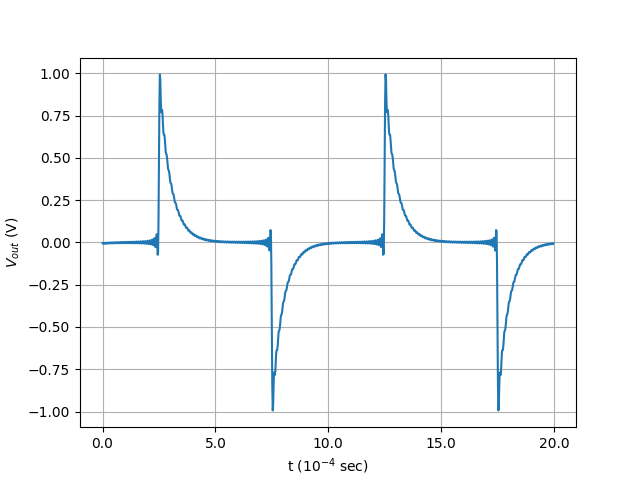
\includegraphics[width = \columnwidth]{2023/PH/37/figs/opt_a_res.png}
        \caption{Opt A: $V_{out}(t)$ vs $t$}
        \label{fig:opt_a_res_gate.ph.23.37}
    \end{figure}
    \newpage
    \item Option B
    \begin{align}
        H_R(j\omega) &=  \frac{R}{R + \frac{1}{j\omega C}}\\
        &= \frac{j\omega RC}{1+j\omega RC}\\
        &= \brak{\frac{\omega R C}{\sqrt{1 + (\omega R C)^2}}}e^{j\tan^{-1}\brak{\frac{1}{\omega RC}}}\label{eq:19_gate.23.ph.37}
    \end{align}
    \begin{figure}[!h]
        \centering
	    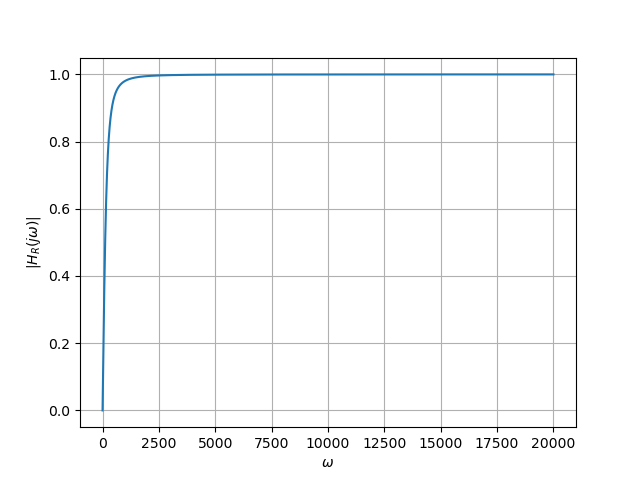
\includegraphics[width=\columnwidth]{2023/PH/37/figs/opt_b_hf.png}
        \caption{$\abs{H_R(j\omega)}$ vs $\omega$ for $R=5k\Omega$, $C=1\mu F$}
        \label{fig:opt_b_hf_gate.ph.23.37}
    \end{figure}
    \begin{align}
        \implies \mathcal{V}_{out}(j\omega) &= H_R(j\omega)\mathcal{V}_{in}(j\omega)
    \end{align}
     Using \eqref{eq:5_gate.23.ph.37} and  \eqref{eq:19_gate.23.ph.37},
    {\small
    \begin{align}
        V_{out}(t) &= \sum_{n=1}^{\infty}\brak{\frac{n\omega R C}{\sqrt{1 + (n\omega R C)^2}}}a_n\cos\brak{n\omega t+\tan^{-1}\brak{\frac{1}{n\omega RC}}}
    \end{align}
    }
    \begin{figure}[!h]
        \centering
        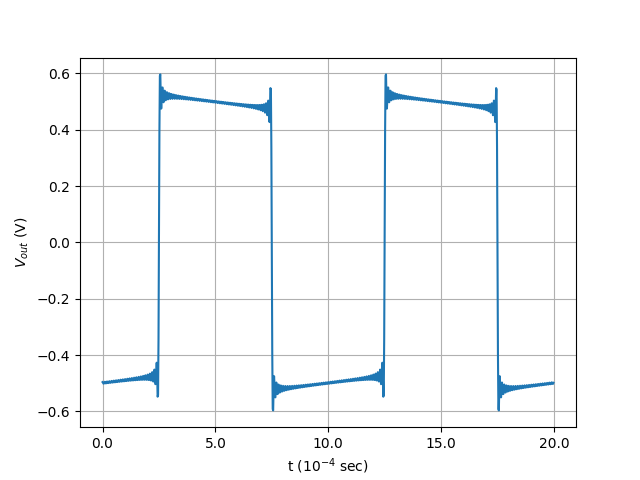
\includegraphics[width = \columnwidth]{2023/PH/37/figs/opt_b_res.png}
        \caption{Opt B: $V_{out}(t)$ vs $t$}
        \label{fig:opt_b_res_gate.ph.23.37}
    \end{figure}
    \item Option C
    \begin{align}
        H_C(j\omega) &=  \frac{\frac{1}{j\omega C}}{R + \frac{1}{j\omega C}}\\
        &= \frac{1}{1+j\omega RC}\\
        &= \brak{\frac{1}{\sqrt{1 + (\omega R C)^2}}}e^{-j\tan^{-1}\brak{\omega RC}}\label{eq:24_gate.23.ph.37}
    \end{align}
    \begin{figure}[!h]
        \centering
        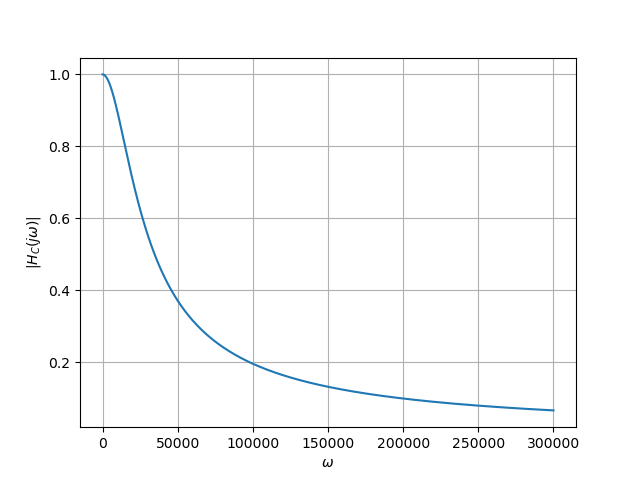
\includegraphics[width=\columnwidth]{2023/PH/37/figs/opt_c_hf.png}
        \caption{$\abs{H_C(j\omega)}$ vs $\omega$ for $R=0.5k\Omega$, $C=0.1\mu F$}
        \label{fig:opt_c_hf_gate.ph.23.37}
    \end{figure}
    \begin{align}
        \implies \mathcal{V}_{out}(j\omega) &= H_C(j\omega)\mathcal{V}_{in}(j\omega)
    \end{align}
     Using \eqref{eq:5_gate.23.ph.37} and  \eqref{eq:24_gate.23.ph.37},
    {\small
    \begin{align}
        V_{out}(t) &= \sum_{n=1}^{\infty}\brak{\frac{1}{\sqrt{1 + (n\omega R C)^2}}}a_n\cos\brak{n\omega t-\tan^{-1}\brak{n\omega RC}}
    \end{align}
    }
    \begin{figure}[!h]
        \centering
        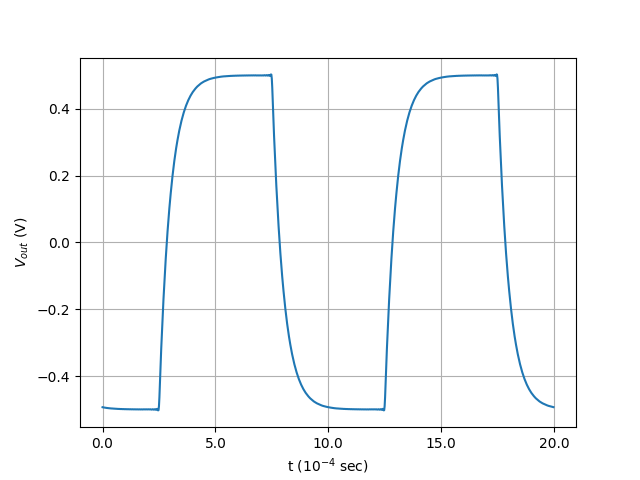
\includegraphics[width = \columnwidth]{2023/PH/37/figs/opt_c_res.png}
        \caption{Opt C: $V_{out}(t)$ vs $t$}
        \label{fig:opt_c_res_gate.ph.23.37}
    \end{figure}
    \item Option D
    \begin{align}
        H_C(j\omega) &=  \frac{\frac{1}{j\omega C}}{R + \frac{1}{j\omega C}}\\
        &= \frac{1}{1+j\omega RC}\\
        &= \brak{\frac{1}{\sqrt{1 + (\omega R C)^2}}}e^{-j\tan^{-1}\brak{\omega RC}}\label{eq:29_gate.23.ph.37}
    \end{align}
    \begin{figure}[!h]
        \centering
        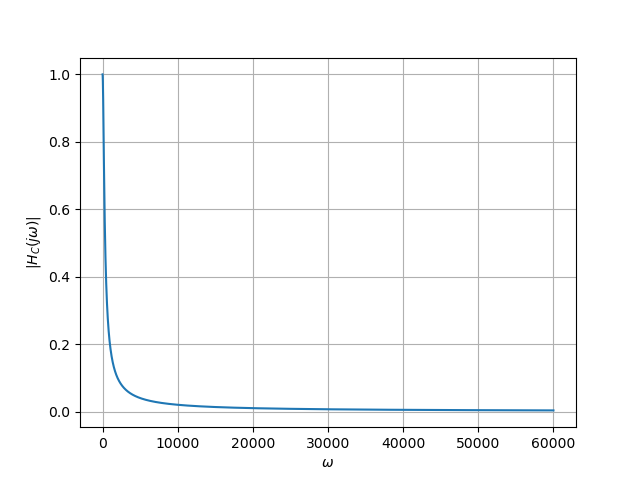
\includegraphics[width=\columnwidth]{2023/PH/37/figs/opt_d_hf.png}
        \caption{$\abs{H_C(j\omega)}$ vs $\omega$ for $R=5k\Omega$, $C=1\mu F$}
        \label{fig:opt_d_hf_gate.ph.23.37}
    \end{figure}
    \begin{align}
        \implies \mathcal{V}_{out}(j\omega) &= H_C(j\omega)\mathcal{V}_{in}(j\omega)
    \end{align}
    Using \eqref{eq:5_gate.23.ph.37} and  \eqref{eq:29_gate.23.ph.37},
    {\small
    \begin{align}
        V_{out}(t) &= \sum_{n=1}^{\infty}\brak{\frac{1}{\sqrt{1 + (n\omega R C)^2}}}a_n\cos\brak{n\omega t-\tan^{-1}\brak{n\omega RC}}
    \end{align}
    }
    \begin{figure}[!h]
        \centering
        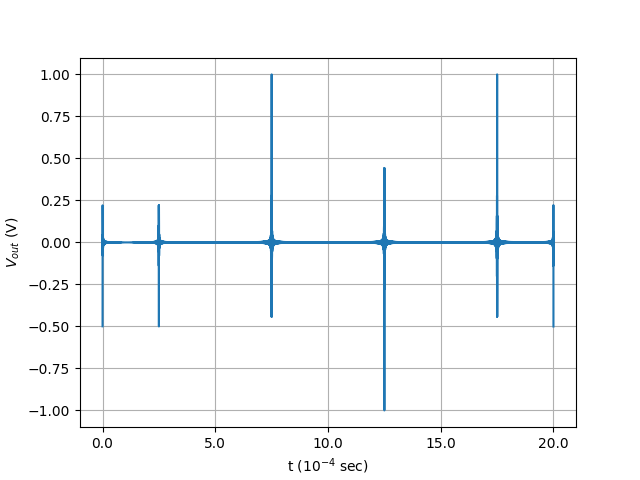
\includegraphics[width = \columnwidth]{2023/PH/37/figs/opt_d_res.png}
        \caption{Opt D: $V_{out}(t)$ vs $t$}
        \label{fig:opt_d_res_gate.ph.23.37}
    \end{figure}
\end{enumerate}
%\end{document}


\pagebreak

\item In the circuit shown below, switch S was closed for long time. If the switch is opened at $t=0$, the  maximum magnitude of the voltage $V_R$ , in volts is (rounded off to the nearest integer)\hfill{(GATE 2023 EC 35)}\\
\begin{figure}[h!]
    \centering
    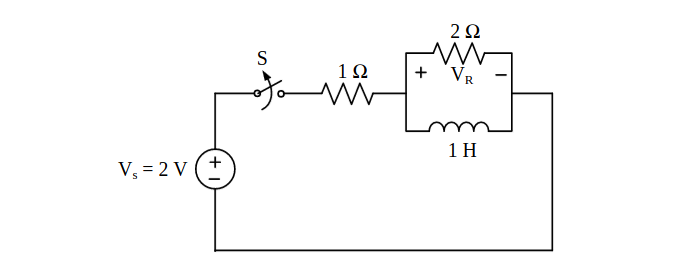
\includegraphics[width=1\linewidth]{2023/EC/35/figs/gate.png}
    \caption{ }
\end{figure}
\solution
\iffalse
\let\negmedspace\undefined
\let\negthickspace\undefined
\documentclass[journal,12pt,twocolumn]{IEEEtran}
\usepackage{cite}
\usepackage{amsmath,amssymb,amsfonts,amsthm}
\usepackage{algorithmic}
\usepackage{graphicx}
\usepackage{textcomp}
\usepackage{xcolor}
\usepackage{txfonts}
\usepackage{listings}
\usepackage{enumitem}
\usepackage{mathtools}
\usepackage{gensymb}
\usepackage{comment}
\usepackage[breaklinks=true]{hyperref}
\usepackage{tkz-euclide} 
\usepackage{listings}
\usepackage{gvv}                                        
\def\inputGnumericTable{}                                 
\usepackage[latin1]{inputenc}                                
\usepackage{color}                                            
\usepackage{array}                                            
\usepackage{longtable}                                       
\usepackage{calc}                                             
\usepackage{multirow}                                         
\usepackage{hhline}                                           
\usepackage{ifthen}                                           
\usepackage{lscape}

\newtheorem{theorem}{Theorem}[section]
\newtheorem{problem}{Problem}
\newtheorem{proposition}{Proposition}[section]
\newtheorem{lemma}{Lemma}[section]
\newtheorem{corollary}[theorem]{Corollary}
\newtheorem{example}{Example}[section]
\newtheorem{definition}[problem]{Definition}
\newcommand{\BEQA}{\begin{eqnarray}}
\newcommand{\EEQA}{\end{eqnarray}}
\newcommand{\define}{\stackrel{\triangle}{=}}
\theoremstyle{remark}
\newtheorem{rem}{Remark}
\usepackage{circuitikz}
\begin{document}

\bibliographystyle{IEEEtran}
\vspace{3cm}

\title{GATE-2023, EC-35}
\author{EE23BTECH11033- JASWANTH KILLANA}
\maketitle
\newpage
\bigskip

\renewcommand{\thefigure}{\theenumi}
\renewcommand{\thetable}{\theenumi}
\textbf{Question}:\\
In the circuit shown below, switch S was closed for a long time. If the switch is opened at t=0, the maximum magnitude of the voltage $V_R$ in volts is. (round off to nearest integer).\\
\begin{figure}[th]
\centering
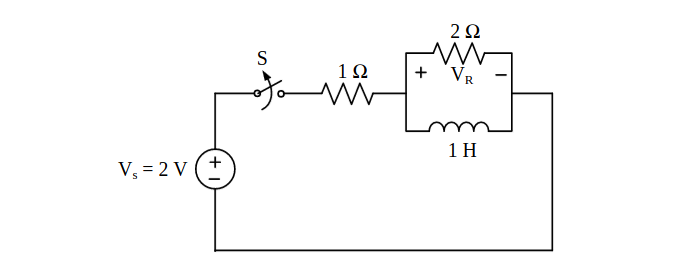
\includegraphics[width=\linewidth]{2023/EC/35/figs/gate.png}
\caption{}
\end{figure}
\textbf{solution} :
\fi
\begin{table}[!ht]
 \centering
  \begin{tabular}{|c|c|c|}
\hline
\textbf{parameter}& \textbf{description}& \textbf{value}
\\\hline
\multirow{3}{1em}\\$i\brak{0^-}$&current at $t<0$ &$2A$
\\\hline
$V_R\brak{t}$&voltage across 2\ohm &-2i\brak{t}u\brak{t}
\\\hline
$L$&inductance&$1H$
\\\hline
$i\brak{t}$& current in small loop after $t=0$&$\frac{V_R\brak{t}}{2}$
\\\hline
$I\brak{s}$& $i\brak{t}$ in laplace &$-$
\\\hline
\end{tabular}



   \caption{input parameters}
   \label{GATE-2023,EC-35}
   \end{table}
 \begin{figure}[h!]
   \centering
   \begin{circuitikz}[american]
       \draw (0,3) to [R,a^=$1\ohm$,v=$V_R$](3,3); 
       \draw (0,3) to [V,a^=$2V$](0,0);
       \draw (3,3) to [short](3,0);
       \draw (0,0) to [short] (3,0);
   \end{circuitikz}
   \caption{steady state circuit}
   \end{figure}
\begin{align}
 At, t=0^-
\end{align}
inductor acts as wire\\
apply KVL 
\begin{align}
-2+1i\brak{0^-}&=0\\
i\brak{0^-}&=2A
\end{align}

   \begin{figure}[h!]
   \centering
   \begin{circuitikz}[american]
       \draw (0,3) to [R,a^=$2\ohm$,v=$V_R$](3,3); 
       \draw (0,0) to [short](0,3);
       \draw (3,3) to [V,a^=$2V$](3,0);
       \draw (0,0) to [L,a^=$Ls$,i=$I\brak{s}$] (3,0);
   \end{circuitikz}
   \caption{s domain circuit fot $t>0$}
   \end{figure}
\begin{align}
2I\brak{s}-2V+LsI\brak{s}&=0\\
\implies I\brak{s}&=\frac{2}{s+2}A
 \end{align}
\begin{figure}[!ht]
     \centering
     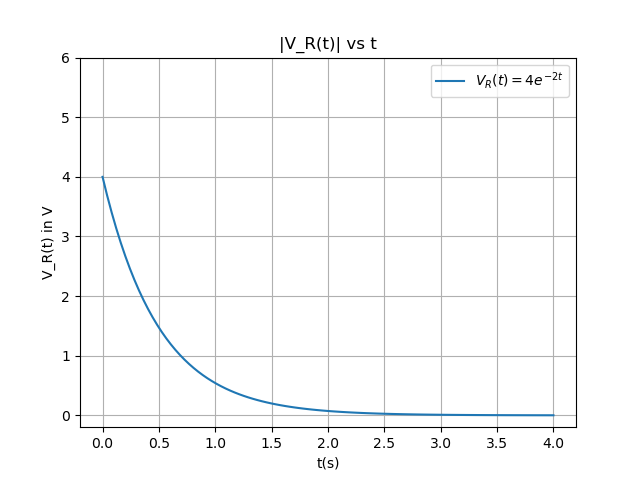
\includegraphics[width=1\linewidth]{2023/EC/35/figs/fig.png}
 \end{figure}
 applying inverse laplace transform
 \begin{align}
  i\brak{t}&=2e^{-2t} u\brak{t}A\\
  V_R\brak{t}&=-2i\brak{t}\\
  \implies V_R\brak{t}&=-4 e^{-2t} u\brak{t}V
 \end{align}  
  As,
 \begin{align}
    t & \xrightarrow{} 0\\
     \implies e^{-2t}&\xrightarrow{} 1\\
     \abs{V_R\brak{max}}&=4V
 \end{align}
%\end{document}

\pagebreak
\item A signal $x\brak{t}=2\cos{(180\pi t)}\cos{(60\pi t)}$ is sampled at 200 Hz and then passed through an ideal low pass filter having cut-off frequency of 100 Hz.\\
The maximum Frequency present in the filtered  signal in Hz is \rule{1cm}{0.5mm} (Round off to the nearest integer.) \hfill (GATE 2023 EE)
\solution
\pagebreak
\item In the circuit shown, the input voltage $V_{in} = 100mV$. The switch and the opamp are ideal. At time $t=0$, the intial charge stored in the $10nF$ capacitor is $1nC$, with the polarity as indicated in the figure. The switch $S$ is controlled using a $1KHz$ square-wave voltage signal $V_s$ as shown. Whenever $V_s$ is `High', $S$ is in position $`1$' and when $V_s$ is `Low', $S$ is in position `$2$'.\\
At $t = 20ms$, the magnitude of the voltage $V_o$ will be  \\  
\begin{figure}[ht]
  \centering
    \resizebox{0.55\columnwidth}{!}{\begin{circuitikz}[american]
    \draw (0,0) node[op amp] (opamp) {};
    \draw (opamp.+) to [short] ++(-1,0) coordinate (leftLine) -- ++(0,-1) node[ground] {};
    \draw (opamp.-) to [short] ++(-1,0) to [short] ++(0,2) to [C, l_={$-$\hspace{1pt}$10nF$\hspace{1pt}$+$}] ++(2,0) to [short] ++(2,0) to [short] ++(0,-2.5);
    \draw (opamp.out) to [short] ++(1.5,0) node[right] {$V_o$};
    \draw (opamp.-) to [short] ++(-2.3,0);
    \draw[thick] ($(opamp.-) + (-2.7,0)$) -- ++(-2.3,0) node[left] (Vin) {$V_{in}$};
    \draw[dotted] ($(Vin.west) + (-1,-0.15)$) -- ($(Vin.west) + (-1,-0.85)$);
    \draw[thick] ($(Vin.west) + (-1,-0.4)$) ++(0,0.15) -- ++(0.5,0) -- ++(0,-0.5)-- ++(0.5,0)  -- ++(0,0.5) -- ++(0.5,0) -- ++(0,-0.5) -- ++(0.5,0) -- ++(0,0.5)  -- ++(0.5,0) -- ++(0,-0.5) -- ++(0.5,0);
    \node[font=\scriptsize] at ($(Vin.west) + (-1.5,-0.15)$) {High};
    \node[font=\scriptsize] at ($(Vin.west) + (-1.5,-0.65)$) {Low};
    \node[font=\scriptsize] at ($(Vin.west) + (-1,-0.85)$) {$t=0$};
    \draw[dotted] ($(Vin.west) + (3.1,0)$) -- ++(0.2,-0.3);
    \draw[dotted] ($(Vin.west) + (3.5,0)$) -- ++(-0.2,-0.3);
    \node[font=\scriptsize] at ($(Vin.west) + (3.3,0) + (0,0.5)$) {S};
    \draw[thick] ($(Vin.west) + (3.3,-0.3)$) -- ++(0,-1) to [C, l=$1nF$] ++(0,-1) node[ground] {};
    \node[font=\scriptsize] at ($(Vin.west) + (3.1,0.15)$) {1};
    \node[font=\scriptsize] at ($(Vin.west) + (3.5,0.15)$) {2};
\end{circuitikz}


}
\end{figure}
\hfill{(GATE IN 2023)}\\
\solution
\pagebreak

\item The value of parameters of the circuit shown in the figure are $R_1=2\ohm$,$R_2=2\ohm$,$R_3=3\ohm$,$L=10 mH$,$C=100\mu F$. For time \(t<0\), the circuit is at steady state with the switch $ 'K'$ in closed condition. If the switch is opened at $t=0$, the value of the voltage across the inductor \brak{V_L}
 at $t=0^{+}$ in Volts is \rule{2cm}{0.4pt} (Round off to 1 decimal place).
\begin{circuitikz}
    \draw (0,0) to [R, R=$R_3$] (0,2);
    \draw (0,3) to [switch, o-o, name=$K$] (0,2);
    \draw (0,3)-- (0,4);
    \draw (0,4) -- (4,4);
    \draw (3,0) to [american current source, l=$10\,\text{A,}\text{DC}$] (3,4);
    \draw (4,4) to (4,5) to (5,5) to[R, l=$R_1$] (6,5);
    \draw (6,5) to(7,5) to[L, l=$L$] (8,5) to (9,5);
    \draw (4,4)to (4,3)to (5,3) to[R, l=$R_2$] (6,3);
    \draw (6,3)to (7,3) to [C, l=$C$] (8,3) to(9,3);
    \draw (9,5) --(9,3);
    \draw (9,4) -- (10,4);
    \draw (10,4)-- (10,0);
    \draw(10,0)--(0,0);
\end{circuitikz} \hfill (GATE 2023 EE 29Q)
\solution
\pagebreak

\item The op amps in the circuit are ideal. The input signals are $V_{S1} = 3 + 0.10 \sin(300t), \text{V}$ and $V_{S2} = -2 + 0.11 \sin(300t)\, \text{V}$. The average value of the voltage $V_0$ is \underline{\hspace{1cm}} volts (rounded off to two decimal places).
\begin{figure}[ht]
\centering
\resizebox{0.55\columnwidth}{!}{\begin{circuitikz}

% Lines
\draw (-2.5,2.5) -- (0.5,2.5);
\draw (0.5,3) -- (0.5,1);
\draw (0.5,1.5) -- (0,1.5);
\draw (0,1.5) -- (0,0);
\draw (-2.5,-4) -- (0.5,-4);
\draw (0.5,-4.5) -- (0.5,-2.5);
\draw (0.5,-3) -- (0,-3);
\draw (0,-3) -- (0,-1.5);
\draw (0.5,3) -- (2,2);
\draw (0.5,1) -- (2,2);
\draw (2,2) -- (3.5,2);
\draw (3.5,2) -- (5.5,2);
\draw (3.5,2) -- (3.5,1.5);
\draw (0.5,-2.5) -- (2,-3.5);
\draw (0.5,-4.5) -- (2,-3.5);
\draw (2,-3.5) -- (3.5,-3.5);
\draw (3.5,-3.5) -- (3.5,-3);
\draw (3.5,-3.5) -- (5.5,-3.5);
\draw (5.5,-3.5) -- (5.5,-2.25);
\draw (5.5,2) -- (5.5,0.75);
\draw (5.5,-0.75) -- (6.5,-0.75);
\draw (0,0) -- (3.5,0);
\draw (0,-1.5) -- (3.5,-1.5);
\draw (6.5,-1.5) -- (6.5,-2.5);
\draw (6.25,-2.5) -- (6.75,-2.5);
\draw (6.3,-2.55) -- (6.7,-2.55);


% Resistors
\draw (3.5,1.5) to [resistor] (3.5,0);
\draw (3.5,0) to [resistor] (3.5,-1.5);
\draw (3.5,-1.5) to [resistor] (3.5,-3);
\draw (5.5,0.75) to [resistor] (5.5,-0.75);
\draw (5.5,-0.75) to [resistor] (5.5,-2.25);

% Labels
\node at (-3,2.5) {$V_{S1}$};
\node at (-3,-4) {$V_{S2}$};
\node at (0.75,2.5) {+};
\node at (0.75,1.5) {-};
\node at (0.75,-3) {-};
\node at (0.75,-4) {+};
\node at (7,-0.75) {$V_o$};
\node at (4.25,0.75) {R};
\node at (4.25,-0.75) {R};
\node at (4.25,-2.25) {R};
\node at (6.25,0) {R};
\node at (6.25,-1.5) {R};
\node at (6.75,-0.8) {+};
\node at (6.75,-1.5) {-};

% Dot 
\filldraw (6.5,-0.75) circle [radius=0.05];
\fill (6.5,-1.5) circle [radius=0.05]; 

\end{circuitikz}

}
\end{figure}
\hfill{(GATE IN 2023)}

\end{enumerate}
